% Created 2021-03-03 Wed 11:16
% Intended LaTeX compiler: pdflatex
\documentclass[english]{article}
\usepackage[T1, T2A]{fontenc}
\usepackage[lutf8]{luainputenc}
\usepackage[english, russian]{babel}
\usepackage{minted}
\usepackage{graphicx}
\usepackage{longtable}
\usepackage{hyperref}
\usepackage{xcolor}
\usepackage{natbib}
\usepackage{amssymb}
\usepackage{amsmath}
\usepackage{caption}
\usepackage{mathtools}
\usepackage{amsthm}
\usepackage{tikz}
\usepackage{grffile}
\usepackage{extarrows}
\usepackage{wrapfig}
\usepackage{rotating}
\usepackage{placeins}
\usepackage[normalem]{ulem}
\usepackage{amsmath}
\usepackage{textcomp}
\usepackage{capt-of}

\usepackage{geometry}
\geometry{a4paper,left=2.5cm,top=2cm,right=2.5cm,bottom=2cm,marginparsep=7pt, marginparwidth=.6in}

 \usepackage{hyperref}
 \hypersetup{
     colorlinks=true,
     linkcolor=blue,
     filecolor=orange,
     citecolor=black,      
     urlcolor=cyan,
     }

\usetikzlibrary{decorations.markings}
\usetikzlibrary{cd}
\usetikzlibrary{patterns}

\newcommand\addtag{\refstepcounter{equation}\tag{\theequation}}
\newcommand{\eqrefoffset}[1]{\addtocounter{equation}{-#1}(\arabic{equation}\addtocounter{equation}{#1})}


\newcommand{\R}{\mathbb{R}}
\renewcommand{\C}{\mathbb{C}}
\newcommand{\N}{\mathbb{N}}
\newcommand{\rank}{\text{rank}}
\newcommand{\const}{\text{const}}
\newcommand{\grad}{\text{grad}}

\theoremstyle{plain}
\newtheorem{axiom}{Аксиома}
\newtheorem{lemma}{Лемма}
\newtheorem{manuallemmainner}{Лемма}
\newenvironment{manuallemma}[1]{%
  \renewcommand\themanuallemmainner{#1}%
  \manuallemmainner
}{\endmanuallemmainner}

\theoremstyle{remark}
\newtheorem*{remark}{Примечание}
\newtheorem*{solution}{Решение}
\newtheorem{corollary}{Следствие}[theorem]
\newtheorem*{examp}{Пример}
\newtheorem*{observation}{Наблюдение}

\theoremstyle{definition}
\newtheorem{task}{Задача}
\newtheorem{theorem}{Теорема}[section]
\newtheorem*{definition}{Определение}
\newtheorem*{symb}{Обозначение}
\newtheorem{manualtheoreminner}{Теорема}
\newenvironment{manualtheorem}[1]{%
  \renewcommand\themanualtheoreminner{#1}%
  \manualtheoreminner
}{\endmanualtheoreminner}
\captionsetup{justification=centering,margin=2cm}
\newenvironment{colored}[1]{\color{#1}}{}

\tikzset{->-/.style={decoration={
  markings,
  mark=at position .5 with {\arrow{>}}},postaction={decorate}}}
\makeatletter
\newcommand*{\relrelbarsep}{.386ex}
\newcommand*{\relrelbar}{%
  \mathrel{%
    \mathpalette\@relrelbar\relrelbarsep
  }%
}
\newcommand*{\@relrelbar}[2]{%
  \raise#2\hbox to 0pt{$\m@th#1\relbar$\hss}%
  \lower#2\hbox{$\m@th#1\relbar$}%
}
\providecommand*{\rightrightarrowsfill@}{%
  \arrowfill@\relrelbar\relrelbar\rightrightarrows
}
\providecommand*{\leftleftarrowsfill@}{%
  \arrowfill@\leftleftarrows\relrelbar\relrelbar
}
\providecommand*{\xrightrightarrows}[2][]{%
  \ext@arrow 0359\rightrightarrowsfill@{#1}{#2}%
}
\providecommand*{\xleftleftarrows}[2][]{%
  \ext@arrow 3095\leftleftarrowsfill@{#1}{#2}%
}
\makeatother
\author{Ilya Yaroshevskiy}
\date{\today}
\title{Практика 2}
\hypersetup{
 pdfauthor={Ilya Yaroshevskiy},
 pdftitle={Практика 2},
 pdfkeywords={},
 pdfsubject={},
 pdfcreator={Emacs 28.0.50 (Org mode )}, 
 pdflang={English}}
\begin{document}

\maketitle
\tableofcontents


\section{Гамма фунция}
\label{sec:orgd35add2}
\[ \int_0^{ + \infty} t^{x - 1}e^{-t}dt = \Gamma(x)\quad, x > 0 \]
\[ \Gamma(n + 1) = n! \]
\[ \int_0^1 t^{x - 1}(1 - t)^{y - 1}dt = B(x, y) = \frac{\Gamma(x)\Gamma(y)}{\Gamma(x + y)} \approx \frac{1}{\binom{x + y}{x}} \]
Формула понижения: \[ \Gamma(x + 1) = x\cdot\Gamma(x) \]
Формула дополнения: \[ \Gamma(x)\Gamma(1-x) = \frac{\pi}{\sin \pi x} \]
\[ \Gamma(\frac{1}{2}) = \sqrt{\pi} \]

\begin{examp}
\[ \int_0^{\frac{\pi}{2}}\sin^{2021}x dx = \left[\begin{array}{l} t = \sin^2 x \\ dt = 2\sin x\cos x dx \\ dx = \frac{dt}{2t^{\frac{1}{2}}(1 - t)^{\frac{1}{2}}}\end{array}\right]  = \int_0^1 t^{1010,5}\cdot\frac{1}{2}t^{-\frac{1}{2}}(1 - t)^{-\frac{1}{2}}dt = \]
\[ = \frac{1}{2} \int_0^1 t^{1010}(1 - t)^{-\frac{1}{2}} dt = \frac{1}{2}B(1011, \frac{1}{2}) = \frac{1}{2}\frac{\Gamma(1011)\Gamma(\frac{1}{2})}{\Gamma(1011 + \frac{1}{2})} = \]
\[ = \frac{1}{2}\frac{1010!\sqrt{\pi}}{\frac{2021}{2}\cdot\frac{2019}{2}\cdot\dots\cdot\frac{1}{2}\cdot\sqrt{\pi}} = \frac{1010!\cdot2^{1009\color{red}?\color{black}}}{2021!!}\]
\end{examp}
\section{Кратные интгералы}
\label{sec:orgb243271}
\begin{center}
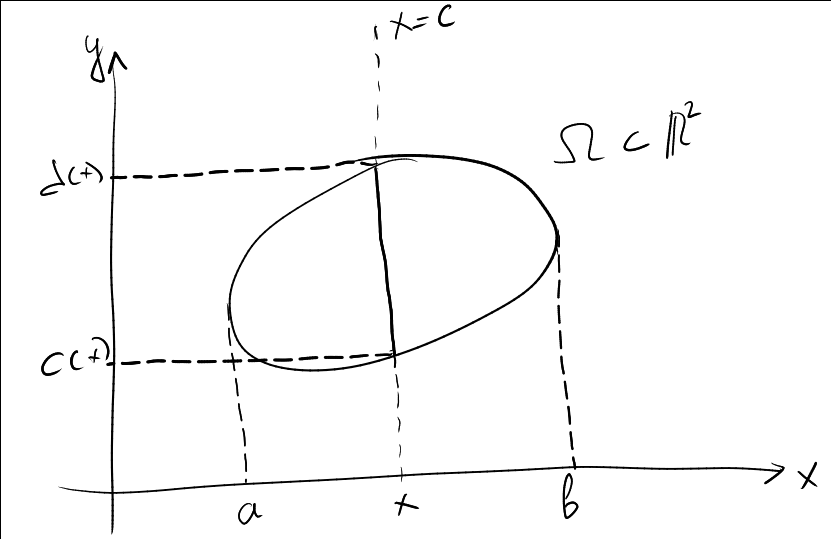
\includegraphics[scale=0.35]{2_1.png}
\end{center}
\[ \iint f dx dy = \int^b_a\left(\int^{d(x)}_{c(x)} f(x, y) dy\right)dx = \]
\[ = \int_C^D\left(\int_{A(y)}^{B(y)}f(x, y) dx\right)dy \]
\begin{center}
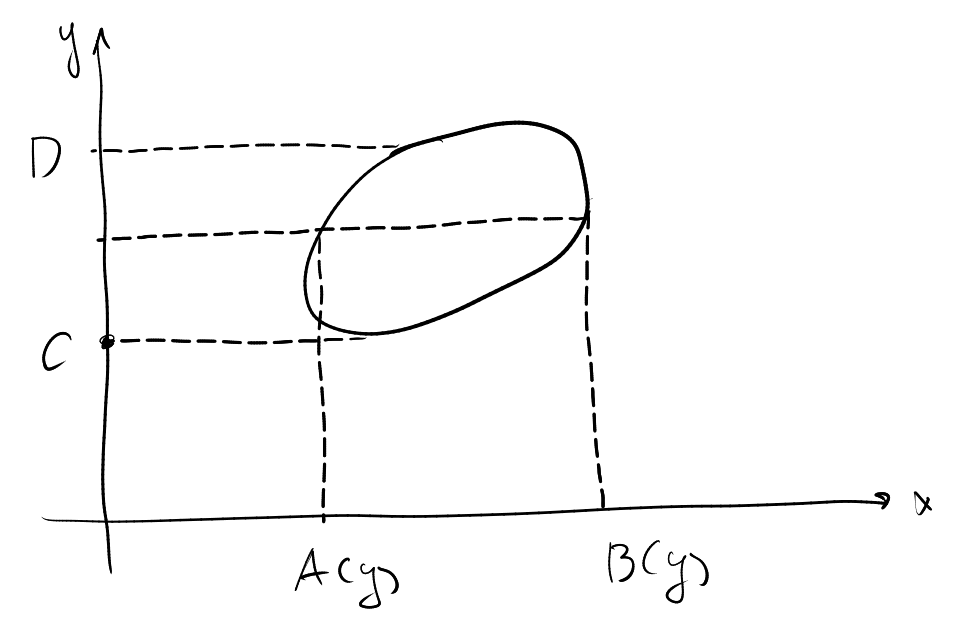
\includegraphics[scale=0.35]{2_2.png}
\end{center}
\begin{examp}
\-
\begin{center}
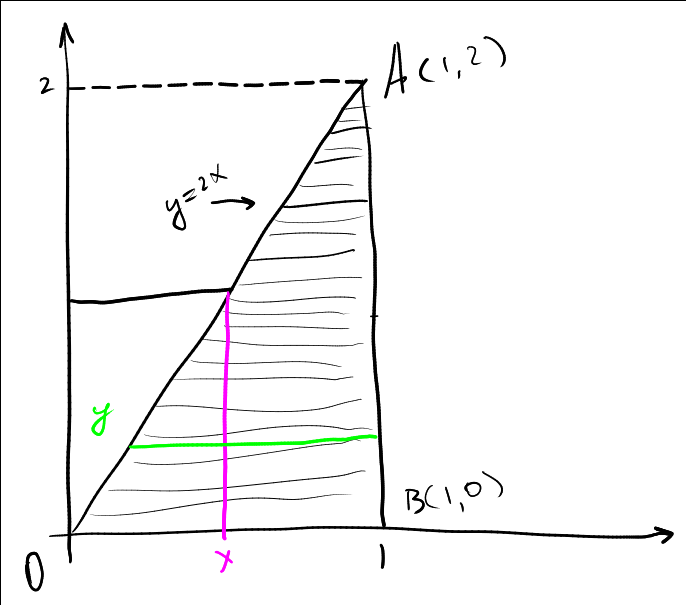
\includegraphics[scale=0.35]{2_3.png}
\end{center}
\[ \iint_{\bigtriangleup AOB} f dx dy = \int_0^1 dx \int_0^{2x} f dy =  \]
\[ = \int_0^2 dy \int_{\frac{y}{2}}^1 f dx \]
\end{examp}

\subsection{Изменение порядка интегрирования}
\label{sec:org9ea45a2}
\[ \int_a^b dx \int^{d(x)}_{c(x)} f dy  \]
\begin{examp}
\[ \iint_{x^2 + y^2 \le y} f dx dy \]
\begin{itemize}
\item \(x^2 + (y - \frac{1}{2})^2 \le \frac{1}{4}\) --- окружность радиуса \(\frac{1}{2}\) с центром в \((0, \frac{1}{2})\)
\end{itemize}
\end{examp}
\begin{examp}
\[ \iint_\Omega f dx dy \]
\begin{center}
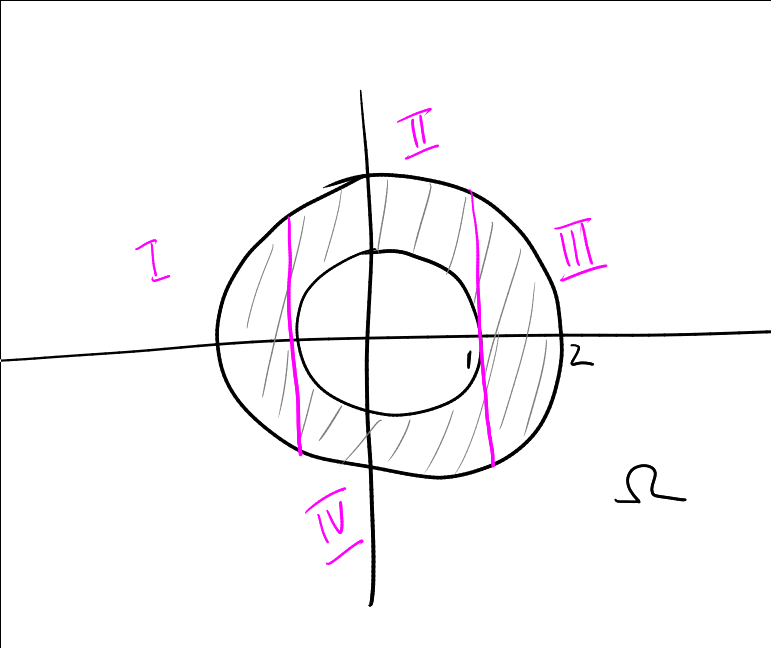
\includegraphics[scale=0.35]{2_4.png}
\end{center}
\[ \color{magenta}I\color{black} = \int^{-1}_{-2} dx \int^{\sqrt{4 - x^2}}_{-\sqrt{4 - x^2}} dy \]
\[ \color{magenta}II\color{black} = \int^1_{-1}dx\int^{\sqrt{4 - x^2}}_{-\sqrt{1 - x^2}} f dy \]
\end{examp}
\begin{examp}
\-
\begin{center}
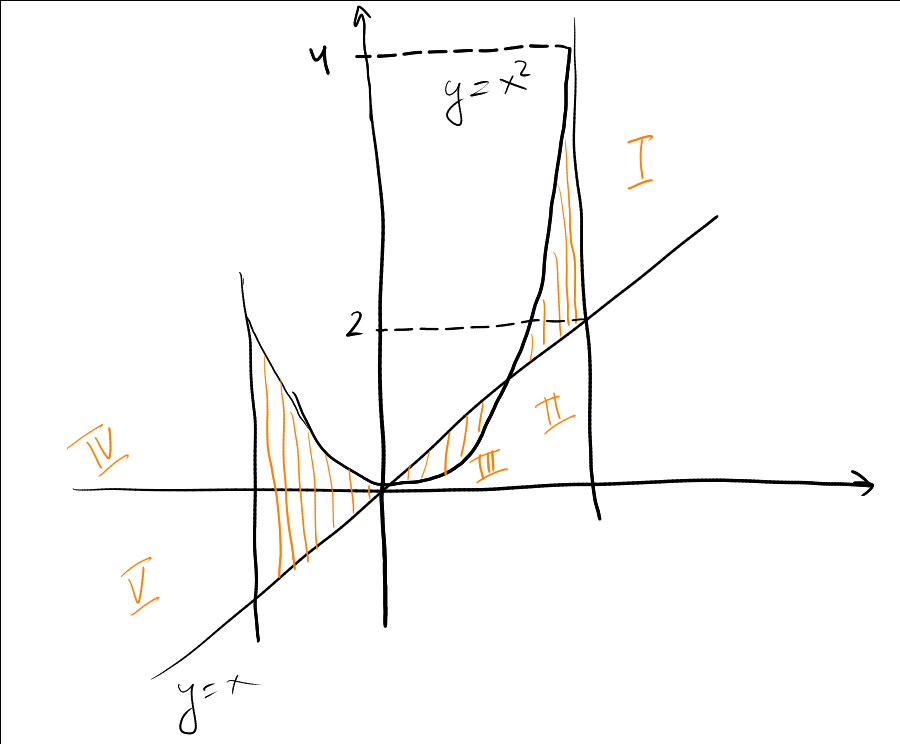
\includegraphics[scale=0.4]{2_5.png}
\end{center}
\[ \int^2_{-1} dx \int^{x^2}_x f dy = \int^4_2 dy \int^2_{\sqrt{y}} f dx + \int^2_1 dy \int^y_{\sqrt{y}} f dx - \int^1_0 dy \int^{\sqrt{y}}_y f dx + \int^1_0 dy \int^{-\sqrt{y}}_{-1} f dx + \int^0_{-1} dy \int^y_{-1} f dx \]
\end{examp}
\end{document}
